\section{Metoda projekcji}
Metoda projekcji jest sposobem indeksowania danych optymalizującym wyznaczanie $ \varepsilon $-otoczenia. Metoda projekcji sposobem działania przypomina metodę nierówności trójkąta.
\subsection{Algorytm wyszukiwania $ \varepsilon $-otoczenia}
Przedstawiany algorytm wyszukiwania $\varepsilon$-otoczenia jest oparty na propozycji \cite{tivsp}. Zakładam, że szukamy $ \varepsilon $-otoczenia punktu $ p $ w zbiorze danych $ D $. Dla każdego punktu $ q \in D $ i wybranej współrzędnej projekcji $ l $ zachodzi zależność, że jeśli różnica wartości współrzędnej projekcji $ l $ punktów $ p $ i $ q $ jest większa niż $ \varepsilon $, to odległość między punktami $ p $ i $ q $ jest również większa od $ \varepsilon $, a stąd punkt $ q $ nie jest elementem $ \varepsilon $-otoczenia punktu $ p $. Projekcja punktu $ q $ na współrzędną \mbox{projekcji $ l $} będzie \mbox{oznaczana $ \pi_l(q) $}. Jeśli dla pewnej miary nie zachodzi \myhyperref{eq:projection-raw}{zależność}, to nie można z tą miarą stosować metody projekcji. 
\begin{equation} \label{eq:projection-raw}
	\abs{\pi_l(p) - \pi_l(q)} > \varepsilon \implies d(p,q) > \varepsilon	\implies q \notin N_{D,\varepsilon}(p)
\end{equation}
Można wywnioskować, że jeśli punkt $ q $ należy do $ \varepsilon $-otoczenia \mbox{punktu $ p $}, to różnica między wartościami współrzędnych punktów $ p $ i $ q $ nie może być większa niż $ \varepsilon $.
\begin{equation}\label{eq:projection}
	q \in N_{D,\varepsilon}(p) \implies d(p,q) \le \varepsilon \implies \abs{\pi_l(p) - \pi_l(q)} \le \varepsilon
\end{equation}
\begin{figure}
	\begin{minipage}[b]{.5\linewidth}
		\centering
		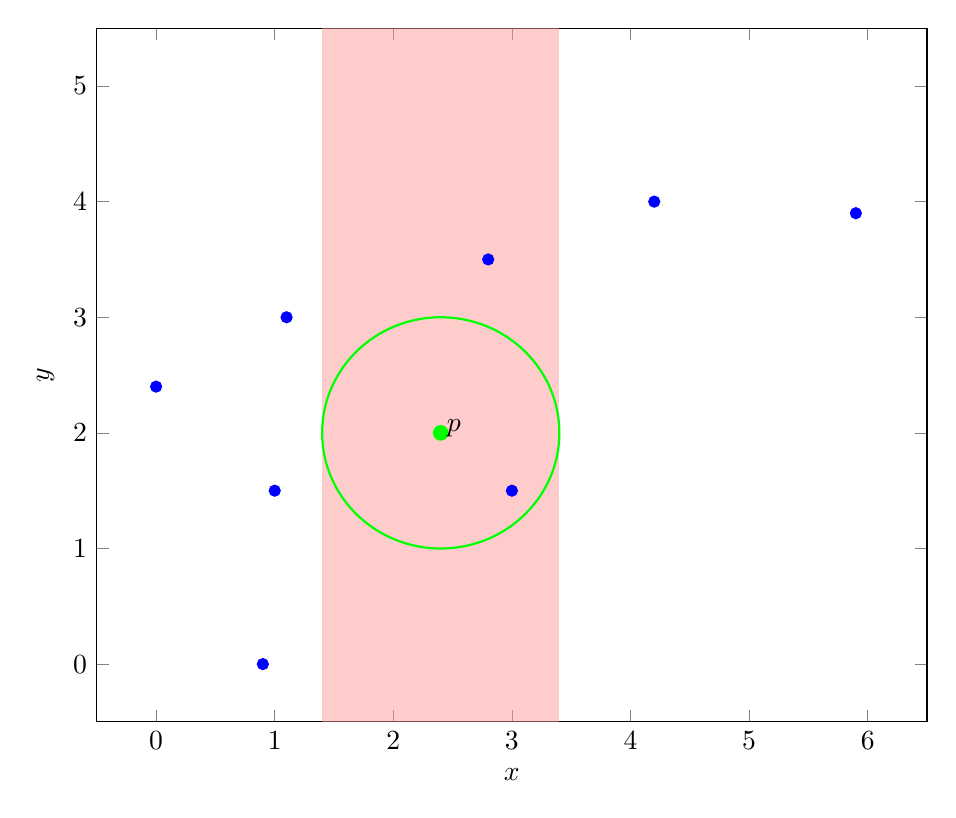
\begin{tikzpicture}[even odd rule]
		\begin{axis}[
		height=0.857\linewidth,
		width=\linewidth,
		xmin=-.5,ymin=-0.5,
		xmax=6.5,ymax=5.5,
		xlabel=$ x $,ylabel=$ y $
		]
		
			
		\def\eps{1}
		\def\Px{2.4}\def\Py{2}
		\coordinate (P) at (\Px,\Py);
		
		\fill[red!40, opacity=.5] (\Px-\eps,-.5) rectangle (\Px+\eps,6.5);
		
		\addplot[blue, only marks] coordinates{ (0.9, 0) (1, 1.5) (0, 2.4) (1.1, 3) (3, 1.5) (2.8, 3.5) (4.2, 4) (5.9, 3.9)  };
		
		\draw[thick, green] (P) circle[radius=\eps];
		\node[green,label={[label distance=-8pt]75:{$ p $}},circle,fill,inner sep=2pt] at (P) {};
		
		\end{axis}
		\end{tikzpicture}
	\end{minipage}%
	\begin{minipage}[b]{.5\linewidth}
		\centering
		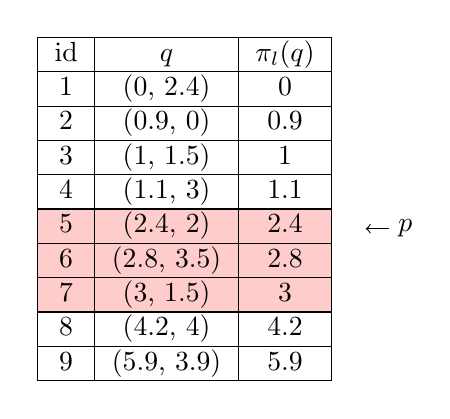
\begin{tikzpicture}
		\node at (0,0) {\begin{tabular}{|c|c|c|}
			\hline 
     id& $ q $ & $ \pi_l(q) $ \\\hline
     	1&(0, 2.4) & 0 \\\hline
			2&(0.9, 0) & 0.9 \\\hline
			3&(1, 1.5) & 1 \\\hline
			4&(1.1, 3) & 1.1 \\\hline
			\rowcolor{red!20}
		  5&(2.4, 2) & 2.4 \\\hline
 			\rowcolor{red!20}
		  6&(2.8, 3.5) & 2.8 \\\hline
 			\rowcolor{red!20}
		  7&(3, 1.5) & 3 \\\hline
			8&(4.2, 4) & 4.2 \\\hline
			9&(5.9, 3.9) & 5.9 \\\hline
			\end{tabular}};
		\draw[<-] (2.3,-.25) -- node[right=4pt] {$ p $} ++(.3,0); 
		\end{tikzpicture}
	\end{minipage}
	\caption{Wyznaczanie $ \varepsilon $-otoczenia punktu $ p=(2.4,2) $ metodą projekcji dla współrzędnej projekcji $ l=x $ i $ \varepsilon = 1$. Czerwonym kolorem oznaczono obszar, w którym wartość współrzędnej $ l $ znajduje się w przedziale $ \left[\pi_l(p)-\varepsilon,\pi_l(p)+\varepsilon\right] $. Zielonym okręgiem oznaczono $ \varepsilon $-otoczenie punktu $ p $. Odległość od punktu $ p $ jest wyznaczana dla punktów 5,6,7. Punkty 4,6 tworzą $ \varepsilon $-otoczenia \mbox{punktu $ p $.}} \label{img:projection}
\end{figure}
Na podstawie $ \myhyperref{eq:projection}{zależności} $ wiemy, że punktów należących do $ \varepsilon $-otoczenia punktu $ p $ należy szukać pośród $ q $ spełniających warunek \mbox{$ \abs{\pi_l(p) - \pi_l(q)} \le \varepsilon $}. Nie każdy punkt $ q $ spełniający warunek $ \abs{\pi_l(p) - \pi_l(q)} \le \varepsilon $ należy do \linebreak$ \varepsilon $-otoczenia punktu $ p $, więc dla każdego takiego punktu $ q $ trzeba sprawdzić, czy spełnia warunek $ d(p,q) \le \varepsilon $. Wartość współrzędnej $ l $ punktów $ q $ spełniających warunek $ \abs{\pi_l(p) - \pi_l(q)} \le \varepsilon $ mieści się w przedziale $ \left[\pi_l(p)-\varepsilon,\pi_l(p)+\varepsilon\right] $.
\begin{equation}
	\abs{\pi_l(p) - \pi_l(q)} \le \varepsilon \implies \pi_l(q) \in \left[\pi_l(p)-\varepsilon,\pi_l(p)+\varepsilon\right]
\end{equation}
Szukamy więc punktów, dla których wartość współrzędnej $ l $ mieści się w przedziale $ \left[\pi_l(p)-\varepsilon,\pi_l(p)+\varepsilon\right] $. Możemy tę wiedzę wykorzystać, aby zapewnić szybki dostęp do zbioru punktów $ q $ spełniających warunek $ \abs{\pi_l(p) - \pi_l(q)} \le \varepsilon $. Należy posortować zbiór danych $ D $ po wartości współrzędnej $ l $. Poszukiwane punkty będą znajdowały się na pozycjach przed oraz po punkcie $ p $. Zaczynając w pozycji punktu $ p $, należy przesuwać się w przód listy i dla każdego kolejnego punktu $ q $ sprawdzać, czy należy do $ \varepsilon $-otoczenia punktu $ p $. Sprawdzanie kończymy, kiedy trafimy na punkt $ q $, dla którego $ \pi_l(q) $ nie mieści się w przedziale $ \left[\pi_l(p)-\varepsilon,\pi_l(p)+\varepsilon\right] $. Analogicznie postępujemy, przesuwając się w tył listy. Wynikiem jest $ \varepsilon $-otoczenie punktu $ p $ zawierające każdy ze sprawdzonych punktów, który spełnia warunek $ d(p,q) \le \varepsilon $ oraz punkt $ p $.

Kompletną metodę projekcji przedstawia \myhyperref{alg:projection}{algorytm}. Wdrożenie metody projekcji do algorytmu DBSCAN ogranicza się do wyboru odpowiedniej współrzędnej projekcji $ l $ i wykonaniu następującego przypisania \linebreak\mbox{$ N_{D,\varepsilon}(p) \gets pjneighbourhood(D, \varepsilon, r, p) $.}

\begin{algorithm}[t]
	\caption{Metoda projekcji}\label{alg:projection}
	
	\DontPrintSemicolon
	
	\SetKwFunction{pjneighbourhood}{pjneighbourhood}
	
	\setcounter{AlgoLine}{0}
	\nonl\SetKwProg{myproc}{Wejście}{}{}
	\myproc{}{
		$ D $ - zbiór danych \;
		$\varepsilon $ - promień otoczenia \;
		$ l $ - współrzędna projekcji \;
		$ p $ - punkt, dla którego jest wyznaczane $ \varepsilon $-otoczenie \;
	}
	\setcounter{AlgoLine}{0}
	\nonl\SetKwProg{myproc}{Wyjście}{}{}
	\myproc{}{
		$ \varepsilon $-otoczenie punktu $ p $\;
	}
	
	\setcounter{AlgoLine}{0}
	\nonl\SetKwProg{myproc}{Definicje}{}{}
	\myproc{}{
		$ sortid(p) $ - pozycja punktu $ p $ w zbiorze $ D $ punktów $ q $ posortowanym według wartości $ \pi_l(q) $\;
		$ at(i) $ - punkt na pozycji $ i $ w zbiorze $ D $ punktów $ q $ posortowanym według wartości $ \pi_l(q) $\;
	}
	\nonl\SetKwProg{myalg}{Algorytm}{}{}
	\myalg{\pjneighbourhood{$D$, $\varepsilon$, $ l $, $ p $}}{
		$ N \gets \set{p}$\;
		$ i \gets sortid(p) - 1$\;
		\While{$ i \ge 1 \land d(at(i), r) \in \left[\pi_l(p)-\varepsilon,\pi_l(p)+\varepsilon\right]$}{
			\lIf{$ d(at(i),p) \le \varepsilon $}{$ N \gets N \cup {at(i)} $}
			$ i \gets i - 1 $\;
		}	
		\While{$ i \le |D| \land d(at(i), r) \in \left[\pi_l(p)-\varepsilon,\pi_l(p)+\varepsilon\right]$}{
			\lIf{$ d(at(i),p) \le \varepsilon $}{$ N \gets N \cup {at(i)} $}
			$ i \gets i + 1 $\;
		}		
		\KwRet{$ N $}
	}
\end{algorithm}

\subsection{Wydajność}
Szukamy $ \varepsilon $-otoczenia punktu $ p $ w zbiorze danych $ D $. Aby zapewnić efektywne działanie \myhyperref{alg:projection}{algorytmu} warto jest wcześniej wyznaczyć wartości projekcji na współrzędną projekcji $ l $ dla każdego punktu $ q $ w zbiorze danych $ D $ \mbox{i odpowiednio} posortować punkty zbioru danych $ D $ względem wartości projekcji na współrzędną $ l $. W ten sposób możemy zapewnić stałą złożoność operacji $ sortid(p) $, $ at(i) $ dla $ i \in \set{1,\dots,|D|} $. Zakładam, że dostęp do wartości $ \pi_l(q) $ dla dowolnego punktu $ q $ posiada stałą złożoność obliczeniową. Jeśli te warunki zostaną spełnione, to możemy przyjąć, że najbardziej czasochłonną operacją \myhyperref{alg:projection}{algorytmu} jest wyznaczanie odległości między punktem $ p $, a punktami $ q $ należącymi do zbioru \mbox{$ R = \set{q | \pi_l(q) \in \left[\pi_l(p)-\varepsilon,\pi_l(p)+\varepsilon\right]} $}.

Jeśli za operację podstawową uznamy obliczanie odległości, to złożoność obliczeniowa wyznaczania $ \varepsilon $-otoczenia za pomocą metody projekcji zależy ściśle od liczebności zbioru $ R $. W pesymistycznym przypadku, dla dostatecznie dużej wartości $ \varepsilon $ liczebność $ R $ może równać się liczebności $ D $. Jeśli założyć, że odwzorowanie zbioru $ D $ na zbiór $ T $ wartości projekcji na współrzędną $ l $ posiada rozkład równomierny, to liczebność zbioru $ R $ można przybliżyć jako stosunek $ \frac{2\varepsilon}{\max(T)-\min(T)} $. 

Wydajność metody projekcji można poprawić, zmniejszając wartość $ \varepsilon $. Wartość $ \varepsilon $ jest jednak parametrem, od którego zależy rezultat algorytmu i nie można go swobodnie zmieniać bez wpływu na wynik. Można za to wpływać na wartość $ m=\max(T)-\min(T) $ bez wpływu na otrzymywane $ \varepsilon $-otoczenie. Wartość $ m $ zależy od doboru współrzędnej projekcji $ l $. Można zatem przyjąć, że powinno się tak dobierać $ l $, żeby maksymalizować wartość $ m $. 

\subsubsection{Wybór współrzędnej projekcji}
Wybór współrzędnej projekcji $ l $ jest decydujący dla wydajności metody projekcji. \myhyperref{img:projection-dim}{Rysunek} ilustruje różne warianty wyboru współrzędnej projekcji. 

\begin{figure}
	\begin{minipage}[b]{.5\linewidth}
		\centering
		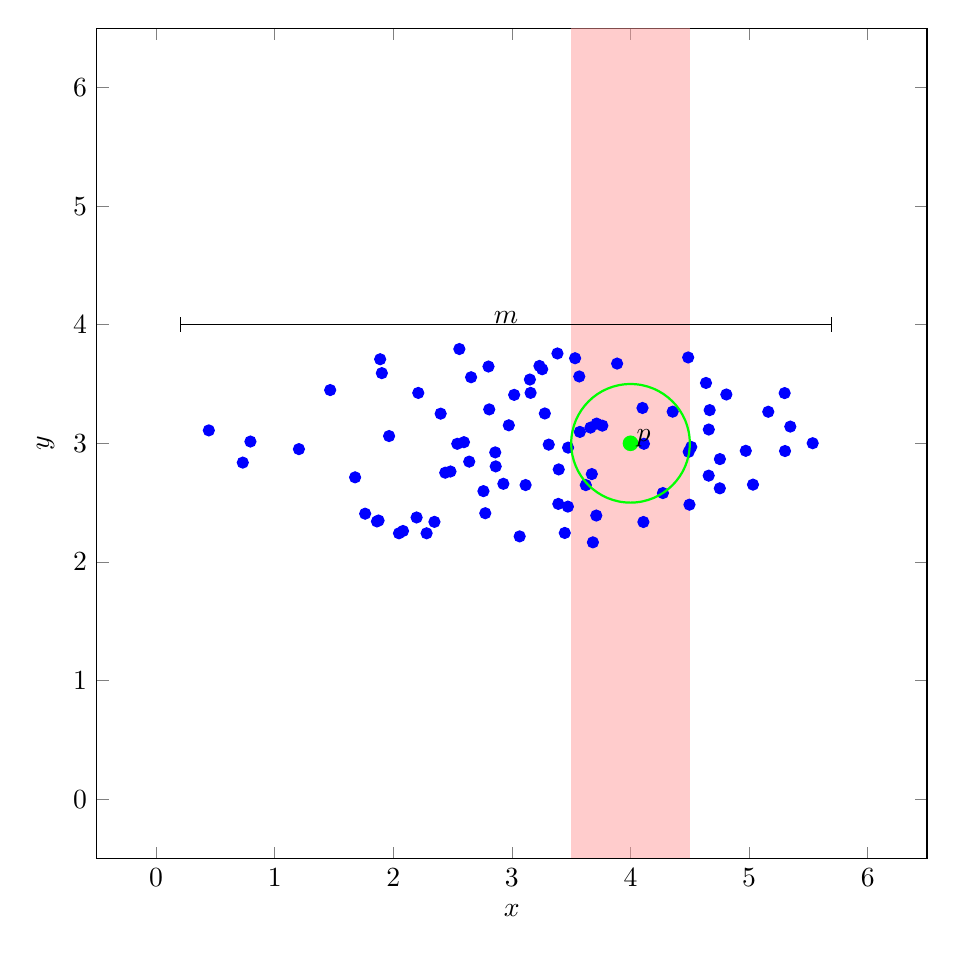
\begin{tikzpicture}[even odd rule]
		\begin{axis}[
		height=\linewidth,
		width=\linewidth,
		xmin=-.5,ymin=-.5,
		xmax=6.5,ymax=6.5, 
		xlabel=$ x $,ylabel=$ y $,
		clip marker paths=true
		]
		
		\def\eps{.5}
		\def\Px{4}\def\Py{3}
		\coordinate (P) at (\Px,\Py);
		
		\fill[red!40, opacity=.5] (\Px-\eps,-.5) rectangle (\Px+\eps,6.5);
		
		\addplot[blue, only marks] coordinates{ (4.75300,2.62048) (3.01900,3.40858) (4.10097,3.29804) (4.48629,3.72395) (2.77545,2.41059) (4.27313,2.58058) (2.34678,2.33772) (5.34738,3.14110) (5.03272,2.65173) (2.28079,2.24148) (2.43791,2.75216) (3.88707,3.67238) (3.47200,2.46638) (4.75376,2.86693) (3.31052,2.98892) (5.53606,3.00095) (1.86217,2.34154) (2.75989,2.59682) (1.88906,3.70902) (2.19653,2.37471) (3.47371,2.96371) (2.80254,3.64745) (4.66737,3.27992) (1.90337,3.59181) (0.73064,2.83741) (2.55698,3.79506) (1.20421,2.95108) (0.44452,3.10897) (3.27753,3.25162) (3.66252,3.13235) (3.44589,2.24428) (5.16155,3.26602) (3.39141,2.48935) (4.63654,3.50896) (3.56788,3.56362) (4.66008,3.11636) (4.97204,2.93688) (1.46772,3.44906) (2.86349,2.80551) (2.80878,3.28588) (3.71428,3.16624) (3.57294,3.09622) (2.04791,2.24134) (4.65917,2.72739) (3.53271,3.71734) (1.96437,3.06133) (4.35553,3.26672) (4.51185,2.96933) (2.39920,3.25011) (3.25534,3.62471) (4.11312,2.99591) (3.71148,2.39100) (2.48199,2.76251) (4.49075,2.92837) (3.15158,3.53781) (4.10860,2.33662) (3.15751,3.42527) (3.67365,2.74072) (2.53914,2.99587) (1.76259,2.40667) (2.92795,2.65857) (2.08172,2.26078) (2.64008,2.84556) (5.30281,2.93501) (3.76251,3.14897) (1.87562,2.34884) (2.21047,3.42493) (3.23212,3.65246) (2.59556,3.00960) (3.11549,2.64829) (5.29967,3.42339) (2.97380,3.15192) (3.68284,2.16500) (3.62310,2.64769) (3.38396,3.75773) (3.06535,2.21522) (3.39482,2.77994) (2.85946,2.92354) (0.79512,3.01500) (2.65582,3.55708) (4.49710,2.48270) (4.80816,3.41169) (1.67785,2.71316) };

		\draw[thick, green] (P) circle[radius=.5];
		\node[green,label={[label distance=-8pt]75:{$ p $}},circle,fill,inner sep=2pt] at (P) {};

		\draw[|-|] (.2,4) -- node[above=-3pt]{$ m $} (5.7,4);
		
		\end{axis}
		\end{tikzpicture}
		\subcaption{$ l=x $}\label{img:projection-dim-good}
	\end{minipage}%
	\begin{minipage}[b]{.5\linewidth}
		\centering
		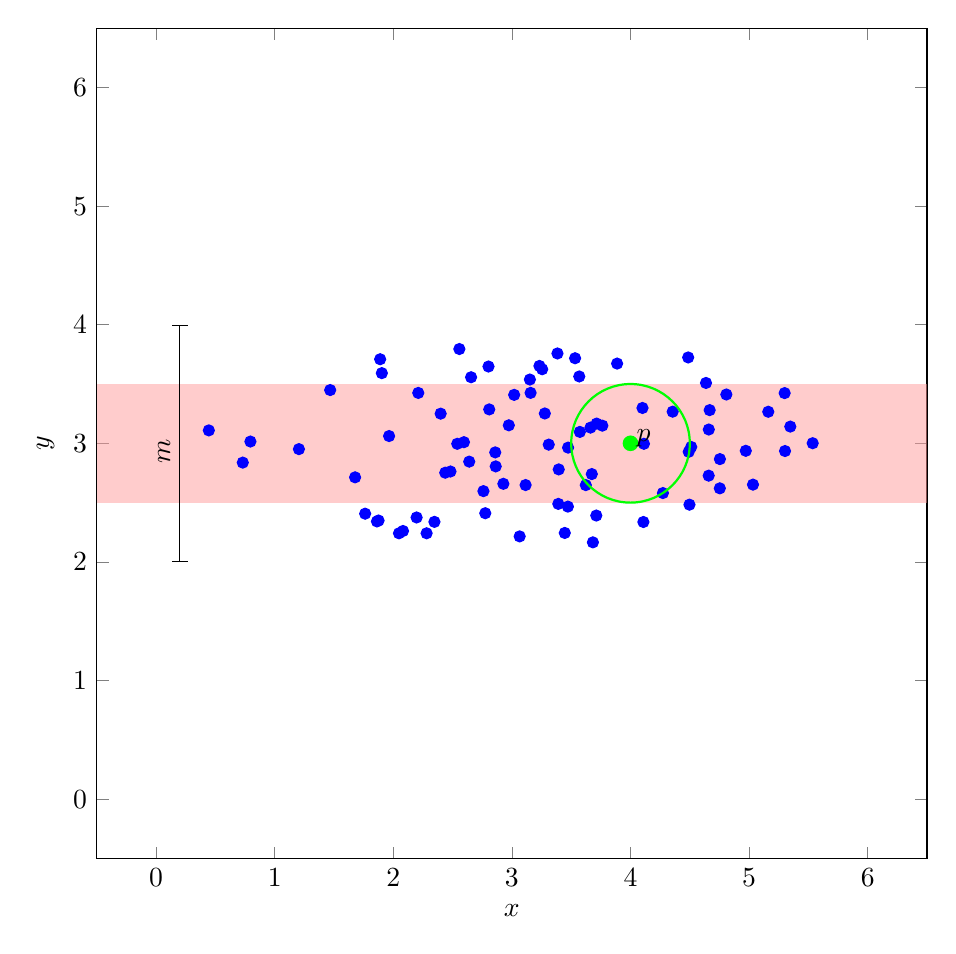
\begin{tikzpicture}[even odd rule]
		\begin{axis}[
		height=\linewidth,
		width=\linewidth,
		xmin=-.5,ymin=-.5,
		xmax=6.5,ymax=6.5, 
		xlabel=$ x $,ylabel=$ y $,
		clip marker paths=true
		]
		
		\def\eps{.5}
		\def\Px{4}\def\Py{3}
		\coordinate (P) at (\Px,\Py);
		
		\fill[red!40, opacity=.5] (-.5,\Py-\eps) rectangle (6.5,\Py+\eps);
		
		\addplot[blue, only marks] coordinates{ (4.75300,2.62048) (3.01900,3.40858) (4.10097,3.29804) (4.48629,3.72395) (2.77545,2.41059) (4.27313,2.58058) (2.34678,2.33772) (5.34738,3.14110) (5.03272,2.65173) (2.28079,2.24148) (2.43791,2.75216) (3.88707,3.67238) (3.47200,2.46638) (4.75376,2.86693) (3.31052,2.98892) (5.53606,3.00095) (1.86217,2.34154) (2.75989,2.59682) (1.88906,3.70902) (2.19653,2.37471) (3.47371,2.96371) (2.80254,3.64745) (4.66737,3.27992) (1.90337,3.59181) (0.73064,2.83741) (2.55698,3.79506) (1.20421,2.95108) (0.44452,3.10897) (3.27753,3.25162) (3.66252,3.13235) (3.44589,2.24428) (5.16155,3.26602) (3.39141,2.48935) (4.63654,3.50896) (3.56788,3.56362) (4.66008,3.11636) (4.97204,2.93688) (1.46772,3.44906) (2.86349,2.80551) (2.80878,3.28588) (3.71428,3.16624) (3.57294,3.09622) (2.04791,2.24134) (4.65917,2.72739) (3.53271,3.71734) (1.96437,3.06133) (4.35553,3.26672) (4.51185,2.96933) (2.39920,3.25011) (3.25534,3.62471) (4.11312,2.99591) (3.71148,2.39100) (2.48199,2.76251) (4.49075,2.92837) (3.15158,3.53781) (4.10860,2.33662) (3.15751,3.42527) (3.67365,2.74072) (2.53914,2.99587) (1.76259,2.40667) (2.92795,2.65857) (2.08172,2.26078) (2.64008,2.84556) (5.30281,2.93501) (3.76251,3.14897) (1.87562,2.34884) (2.21047,3.42493) (3.23212,3.65246) (2.59556,3.00960) (3.11549,2.64829) (5.29967,3.42339) (2.97380,3.15192) (3.68284,2.16500) (3.62310,2.64769) (3.38396,3.75773) (3.06535,2.21522) (3.39482,2.77994) (2.85946,2.92354) (0.79512,3.01500) (2.65582,3.55708) (4.49710,2.48270) (4.80816,3.41169) (1.67785,2.71316) };

		\draw[thick, green] (P) circle[radius=.5];
		\node[green,label={[label distance=-8pt]75:{$ p $}},circle,fill,inner sep=2pt] at (P) {};

		\draw[|-|] (.2,2) -- node[above=-3pt,rotate=90]{$ m $} (.2,4);
		
		\end{axis}
		\end{tikzpicture}
		\subcaption{$ l=y $}\label{img:projection-dim-bad}
	\end{minipage}
	\caption{Wyznaczanie $ \varepsilon $-otoczenia punktu $ p $ dla różnych wariantów wyboru współrzędnej projekcji $ l $ oraz $ \varepsilon=0.5 $. Punkty znajdujące się w czerwonym obszarze wymagają wyznaczenia odległości od $ p $.}\label{img:projection-dim}
\end{figure}

Jednym ze sposobów na wybranie efektywnej współrzędnej projekcji $ l $ jest wybranie takiego $ l $, dla którego wartość $ m $ jest największa. Wyznaczenie wartości $ m $ dla danego $ l $ jest realizowalne w czasie liniowym, ale możliwych do wyboru współrzędnych jest $ dim(D) $. Wyznaczenie wartości $ m $ dla wszystkich współrzędnych nie powinno stwarzać problemów wydajnościowych nawet dla wysokowymiarowych danych.

\begin{table}[H] 
	\footnotesize
	\tabcolsep=0.11cm
	\centering
	\begin{tabular}{|c|c|c|c|c|c|c|c|c|c|c|c|c|c|c|c|c|}
		\hline 
	$D$			&$ \varepsilon $ & $ \mu $ & $|D|$&$dim(D)$&$l$&$m$&$mad$&$sd$&$T_s [s]$&$T[s]$\\\hline
	seqoia	&4000	&4&62556	&2	&1	&1.04e+06&1.19e+05	&1.44e+05&0.09&0.65		\\\hline
	seqoia	&4000	&4&62556	&2	&0	&1.32e+06&2.74e+05	&3.21e+05&0.09&1.30		\\\hline
	birch		&4000	&4&100000	&2	&1	&1.00e+06&2.31e+05	&2.66e+05&0.13&1.95		\\\hline
	birch		&4000	&4&100000	&2	&0	&9.95e+05&2.31e+05	&2.66e+05&0.09&1.94		\\\hline
	cup98		&40		&4&96367	&56	&37	&6.00e+03&6.59e+03	&9.40e+03&0.12&45.07	\\\hline
	cup98		&40		&4&96367	&56	&25	&6.50e+02&3.61e+01	&5.00e+01&0.10&494.01	\\\hline
	covtype	&120	&4&50000	&55	&5	&7.12e+03&1.29e+03	&1.56e+03&0.07&10.36	\\\hline
	covtype	&120	&4&50000	&55	&0	&1.97e+03&2.18e+02	&2.81e+02&0.09&68.75	\\\hline
	\end{tabular}
	\caption{Grupowania zbioru danych $ D $ algorytmem DBSCAN z metodą projekcji. $ mad $ - średnie bezwględne odchylenie współrzędnej $ l $, $ sd $ - odchylenie standardowe współrzędnej $ l $, $ T_s $ - czas sortowania, $ T $ - całkowity czas grupowania}\label{tbl:projection-time-by-dim}
\end{table}
Doświadczenia pokazują, że dobrymi wskaźnikami efektywności wybranej współrzędnej projekcji mogą też być wartości odchylenia standardowego lub bezwzględnego średniego odchylenia, przy czym należy te wartości maksymalizować. \myhyperref{tbl:projection-time-by-dim}{Tabela} przedstawia przykłady czasu grupowania rzeczywistych zbiorów danych w zależności od wartości wskaźników dla wybranej współrzędnej projekcji $ l $.

\subsubsection{Wiele wymiarów projekcji}
Istnieje wariant metody projekcji, który umożliwia wykorzystanie wielu współrzędnych projekcji. Zakładam, że wyznaczane jest $ \varepsilon $-otoczenie punktu $ p $ w zbiorze danych $ D $. Metoda projekcji z wieloma wymiarami projekcji działa podobnie jak zwykła metoda projekcji. Nadal wymagane jest wybranie współrzędnej projekcji $ l $, po którym sortowane są dane. Dodatkowo wybierany jest jeszcze zbiór innych współrzędnych $ L $. Różnica w działaniu algorytmu polega na tym, że dodatkowo wprowadza się \myhyperref{eq:projection-mult}{warunek} na przynależność punktu $ q $ do $ \varepsilon $-otoczenia $ p $.
\begin{equation}\label{eq:projection-mult}
	q \in N_{D,\varepsilon}(p) \implies  \forall_{\lambda\in L}\,\pi_\lambda(q) \in \left[\pi_\lambda(p)-\varepsilon,\pi_\lambda(p)+\varepsilon\right] 
\end{equation}
Dzięki wprowadzeniu \myhyperref{eq:projection-mult}{warunku} możemy uniknąć wyznaczania dystansu dla części punktów. \myhyperref{tbl:projection-time-by-nu}{Tabela} pokazuje, że zastosowanie wielu wymiarów projekcji może dać wymierny zysk.

\begin{table}[H] 
	\footnotesize
	\tabcolsep=0.11cm
	\centering
	\begin{tabular}{|c|c|c|c|c|c|c|c|c|c|c|c|}
		\hline 
		$D$			&$ \varepsilon $ & $ \mu $ & $|D|$&$dim(D)$& $ mad_1 $&$ mad_2 $&$ mad_3 $&$ T_s[s]$&$ T_1[s] $&$ T_2[s] $&$ T_3[s] $\\\hline
		seqoia	&4000	&4&62556	&2 &273802&119222&-& 0.09 & 0.75  & 0.44 		& -		\\\hline
		birch		&4000	&4&100000	&2 &230514&230517&-& 0.14 & 2.07  & 1.03		& -		\\\hline
		cup98		&40		&4&96367	&56&659&635&36& 0.13 & 44.53 & 32.93		& 27.00		\\\hline
		covtype	&120	&4&100000	&55&1292&998&216& 0.15 & 44.29 & 11.494	& 9.021	\\\hline
	\end{tabular}
	\caption{Grupowania zbioru danych $ D $ algorytmem DBSCAN z metodą projekcji z $ \nu $ współrzędnymi projekcji, $ \nu \in \set{1,2,3} $. Wybrano $ \nu $ współrzędnych projekcji o najwyższej wartości średniego bezwzględnego odchylenia. Dane zostały posortowane po współrzędnej projekcji o maksymalnej wartości średniego bezwzględnego odchylenia. $ mad_i $ - średnie bezwględne odchylenie $ i $-tej współrzędnej projekcji, $ T_s $ - czas sortowania, $ T_\nu $ - całkowity czas grupowania z $ \nu $ współrzędnymi projekcji}\label{tbl:projection-time-by-nu}
\end{table}

\begin{algorithm}[t]
	\caption{Metoda projekcji z wieloma współrzędnymi projekcji}\label{alg:projection-mult}
	
	\DontPrintSemicolon
	
	\SetKwFunction{multpjneighbourhood}{multpjneighbourhood}
	
	\setcounter{AlgoLine}{0}
	\nonl\SetKwProg{myproc}{Wejście}{}{}
	\myproc{}{
		$ D $ - zbiór danych \;
		$\varepsilon $ - promień otoczenia \;
		$ l $ - współrzędna projekcji \;
		$ L $ - zbiór dodatkowych współrzędnych projekcji\;
		$ p $ - punkt, dla którego jest wyznaczane $ \varepsilon $-otoczenie \;
	}
	\setcounter{AlgoLine}{0}
	\nonl\SetKwProg{myproc}{Wyjście}{}{}
	\myproc{}{
		$ \varepsilon $-otoczenie punktu $ p $\;
	}
	
	\setcounter{AlgoLine}{0}
	\nonl\SetKwProg{myproc}{Definicje}{}{}
	\myproc{}{
		$ sortid(p) $ - pozycja punktu $ p $ w zbiorze $ D $ punktów $ q $ posortowanym według wartości $ \pi_l(q) $\;
		$ at(i) $ - punkt na pozycji $ i $ w zbiorze $ D $ punktów $ q $ posortowanym według wartości $ \pi_l(q) $\;
	}
	\nonl\SetKwProg{myalg}{Algorytm}{}{}
	\myalg{\multpjneighbourhood{$D$, $\varepsilon$, $ l $, $ L $, $ p $}}{
		$ N \gets \set{p}$\;
		$ i \gets sortid(p) - 1$\;
		\While{$ i \ge 1 \land d(at(i), r) \in \left[\pi_l(p)-\varepsilon,\pi_l(p)+\varepsilon\right]$}{
			\If{$ \forall_{\lambda\in L}\,\pi_\lambda(at(i)) \in \left[\pi_\lambda(p)-\varepsilon,\pi_\lambda(p)+\varepsilon\right]  $}{
					\lIf{$ d(at(i),p) \le \varepsilon $}{$ N \gets N \cup {at(i)} $}
			}
			$ i \gets i - 1 $\;
		}	
		\While{$ i \le |D| \land d(at(i), r) \in \left[\pi_l(p)-\varepsilon,\pi_l(p)+\varepsilon\right]$}{
			\If{$ \forall_{\lambda\in L}\,\pi_\lambda(at(i)) \in \left[\pi_\lambda(p)-\varepsilon,\pi_\lambda(p)+\varepsilon\right]  $}{
				\lIf{$ d(at(i),p) \le \varepsilon $}{$ N \gets N \cup {at(i)} $}
			}
			$ i \gets i + 1 $\;
		}		
		\KwRet{$ N $}
	}
\end{algorithm}